\cleardoublepage
\chapter{Monte Carlo}\label{chap:app2}

In this appendix we will try to explain the code of the simulation program, which uses the Monte Carlo method to calculate the geometric efficiency of the detectors. In this case we have used the C programming language. This appendix also explains the geometry of the system, which is shown in Fig. \ref{fig:app2}. The code is included at the end.

The first lines of code ask for the input data (the distance between scintillators and the number of muons to be simulated). The dimensions of the scintillators are fixed to 10$\times$31 cm, which are the dimensions of the scintillators at the lab. The algorithm is as follows:

\ben
	\item The program generates a stream of particles through a \code{for} loop, where they are simulated one by one. Each particle strikes the upper detector in random positions given by the triad $(x, y, z)$, that follow a random angular distribution typical of cosmic radiation, given by $cos^4\theta$\footnote{Where $\theta$ is defined in spherical coordinates.} (Appendix \ref{chap:app1}).

	\item For the random number generation, the program uses the C function \code{rand()}, which generates random numbers with values between 0 and \code{RAND\_MAX} = 32768. According to Fig. \ref{fig:app2}, the initial positions on the scintillator 1 are given by:
	\bi
		\item $x \in [0, x_s]$, where $x_s$ is the width of the scintillator, so $x = x_srand()$
		\item $y \in [0, y_s]$, where $y_s$ is the length of the scintillator, so $y = y_srand()$
		\item $z = d$, where $d$ is the distance between scintillators.
	\ei

	\item Then, the direction of incidence ($\theta$, $\varphi$) is generated. This is the direction whith which the particle exits the first detector. It must be taken into account that the angle $\theta$ grows from $-\pi / 2$ to $+\pi / 2$\footnote{This is the incidence angle. Note that there is symmetry between what goes above and below the scintillator.}. The muon reaches the second detector at position $(x', y', z')$. If the projection of $(x, y, z)$ on the plane is given by $\rho$, the projection on the plane from point $P$ to point $P'$ is $\rho''$, which depends on the direction of incidence as:

	\bc$\rho' = d\,\tan\theta$\ec

where $\tan\theta$ is calculated from a $\cos\theta$ generated as the fourth root of a random number between 0 and 1 (App. \ref{chap:app1}), so that we give the correct angular weight to our distribution:

	\bc
		$\cos\theta = \sqrt[4]{\code{rand()}}$

		$\sin^2\theta = \sqrt{1 - \cos^2\theta} \quad \rightarrow \quad$
		$\tan\theta = \frac{\sqrt{1 - \cos^2\theta}}{cos\theta}$
	\ec

Since the system has azimuthal isotropy, the $\varphi$ coordinate is generated in the following way:

	\bc $\varphi \in [0, 2\pi], \quad \rightarrow \quad \varphi = 2\pi\,\code{rand()}$ \ec

	\item After crossing the lower scintillator, the impact point is simulated. The position of the particle in the lower detector is given by the sum of two vectors, one is the projection of the initial position $(x, y, z)$ on the plane ($\rho$), and the other is the vector $\rho'$ mentioned above, as shown in Fig. \ref{fig:app2}, so that its new coordinates on the second scintillator will be:

	\begin{equation*}
		\begin{split}
			x' &= x + \rho'cos\varphi\\
			y' &= y + \rho'sen\varphi\\
			z' &= 0.
		\end{split}
	\end{equation*}

	\item Once the new positions on the lower detector are calculated, they may fall within or outside its limits depending on the angular distribution they have. Applying the correct condition, the program will count how many times it succeeds in collecting each particle. This condition is:

	\graybox{.8}{.7}{\enquote{If $x \in [0, x_s]$, and $y \in [0, y_s]$, (that is, if the two conditions are fulfilled simultaneously) then count one.}}

The value of the counts is stored in a variable with each iteration of the \code{for} loop, and when the loop is finished the program calculates the geometric efficiency as the ratio between this variable and the initial number of particles.
\een

	\bfi[H]
		\bc
			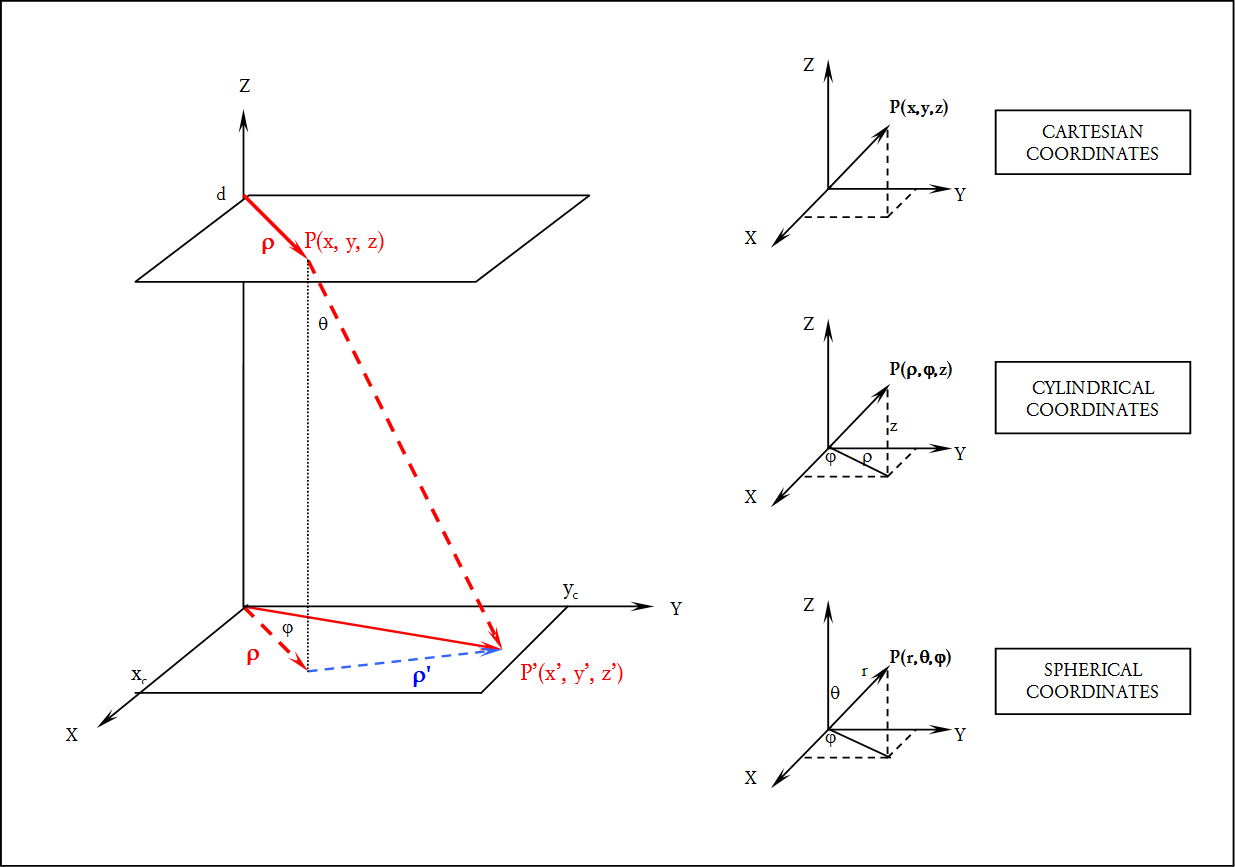
\includegraphics[width=.9\textwidth]{img/app2.png}
			\caption
				[geometry used to simulate the setup used in the laboratory.]
				{On the left, the geometry used to simulate the setup used in the laboratory. The coordinates of a particle that arrives to the upper detector at point $P$, and then moves to point $P'$ of the lower detector, are a combination of Cartesian, Cylindrical and Spherical coordinates. The angular coordinate $\theta$ shown in the figure on the left is the angle of incidence, not to be confused with the coordinate $\theta$ of the Spherical coordinates.}\label{fig:app2}
		\ec
	\efi

Once the efficiency is calculated for one detector, it is known for the other, since we made the approximation that the scintillators are similar.

In the case of an \textit{isotropic distribution}, the problem's geometry does not change, only the angular distribution, and the same program can be used modifying the line:
	
\lstinputlisting[
	firstnumber = 49,
	firstline   = 49,
	lastline    = 49
]{../mcEff/mcScin.c}

for:

\lstinputlisting[
	firstnumber = 49,
	firstline   = 49,
	lastline    = 49
]{../mcEff/mcScinIso.c}

Below, the code is shown:

\lstinputlisting{../mcEff/mcScin.c}

